\documentclass[12pt]{article}
\usepackage[papersize={8.5in,11in}]{geometry}
\usepackage[pdftex]{graphicx}
\DeclareGraphicsExtensions{.pdf,.png,.jpg}
%
\usepackage{amsmath}
\usepackage{amsthm}
\usepackage{amssymb}
\usepackage{textcomp}
\usepackage[all]{xy}
\usepackage{fancyhdr}
\usepackage{hyperref}
\usepackage{verbatim}
\usepackage{algorithm}
\usepackage{algorithmic}
\usepackage{color}
\usepackage[usenames,dvipsnames,svgnames,table]{xcolor}
\usepackage{rotating}
\usepackage{wrapfig}
\usepackage{tikz}
\usetikzlibrary{shapes.geometric, arrows}
\usepackage{framed}

\usepackage{listings}
\lstset{language=python,frame=ltrb,framesep=5pt,basicstyle=\normalsize,
 keywordstyle=\ttfamily\color{DarkRed},
%morecomment=[n][\textbf]{In\ [}{]\:},
%morecomment=[n][\textbf]{Out\ [}{]\:},
morecomment=[s][\color{blue}]{In\ [}{]\:},
morecomment=[s][\color{red}]{Out[}{]\:},
identifierstyle=\ttfamily\color{DarkBlue}\bfseries,
commentstyle=\color{OliveGreen},
stringstyle=\ttfamily,
showstringspaces=false,tabsize = 3}

\lstdefinelanguage{shell} {
commentstyle = \color{black},
keywordstyle = \color{black},
stringstyle = \color{black},
identifierstyle = \color{black},
morecomment=[s][\color{blue}]{In\ [}{]\:},
morecomment=[s][\color{red}]{Out[}{]\:},
 }


%
% this gives a little box for the end of a proof:
%
\def\endthrmbox{$\sqsubset \!\!\!\! \sqsupset$}

\newcommand{\dis}{\displaystyle}
 \def      \RR             {{\mathbb R}}
        \def      \NN             {{\Bbb N}}
        \def      \QQ             {{\Bbb Q}}
        \def      \CC             {{\Bbb C}}
        \def      \ZZ             {{\Bbb Z}}


        \def       \a              {{\alpha}}
        \def       \b              {{\beta}}
        \def       \d              {{\delta}}
        \def       \D              {{\Delta}}
        \def         \e              {{\varepsilon}}
        \def         \g              {{\gamma}}
        \def         \G              {{\Gamma}}
        \def       \l              {{\lambda}}
        \def       \L              {{\Lambda}}
        \def        \m               {{\mu}}
        \def         \n              {{\nabla}}
        \def       \var          {{\varphi}}
        \def         \s              {{\sigma}}
        \def       \Sig          {{\Sigma}}
        \def       \Om          {{\Omega}}

        \def       \t              {{\tau}}
        \def         \th             {{\theta}}
        \def       \O              {{\Omega}}
        \def       \o              {{\omega}}
        \def         \z              {{\zeta}}
       \def        \P             {{\Phi}}
       \def        \p             {{\phi}}
        %Other macros

        \def       \iy              {{\infty}}
        \def         \pa             {{\partial}}
        \def         \div           {{\rm div}}
         \def       \na            {{\nabla}}


%\renewcommand\baselinestretch{1.3}
%% The following block is for narrow margins:
\setlength{\topmargin}{-0.9in}
\setlength{\textheight}{9.50in}
\setlength{\oddsidemargin}{-0.375in}
\setlength{\evensidemargin}{-0.375in}
\setlength{\textwidth}{7.25in}
\setlength{\parindent}{0pt}
\setlength{\parskip}{2pt}
%% end page descript.




\usepackage[compact,explicit]{titlesec}
\titleformat{\section}[runin]{\large\bfseries}{}{0pt}{\titlerule[1.5pt]\newline\vspace*{-4pt} Problem\quad\thesection\newline}[\vspace{0.01ex}{\titlerule[1.5pt]}]

\usepackage[final]{pdfpages}


\title{Homework \#1}
\author{Kyle MacMillan}


\begin{document}
\maketitle

I'm aware that any ``paper'' wouldn't contain the word ``I''. ``I'' is used 
extensively throughout this paper because I wanted to focus on what \textit{I} 
did and I was not interested in skirting around the language to find clever ways 
to say things without including ``I''. 

\section{} %%  This will generate a numbered problem header.

\subsection{Statement}
Compare the effectiveness of the text's hill climbing (two) and simulated annealing algorithms to find the max of
$$
f(x)=2^{-2((x-0.1)/0.9)^2}(\sin(5\pi x))^6 \quad
   \mbox{with} \quad x\in [0,1].
$$

Use a real valued representation.  Include a plot of the function with the 
location of the max and a plot of the estimate as a function of the iteration 
number. How sensitive are the algorithms to initial values?

\subsection{Method}

$$$$
I built the Hill Climb algorithm according to page 65 in the text. At first I 
had trouble getting anything to work because I wasn't familiar with parallel 
arrays in numpy. After fixing the bouncing fitness issues (due to parallel array 
sorting) I had to figure out how to perturb the data. 

$$$$
I decided on a simple mutation to each $x$ value, recombination was skipped. I 
played around with perturbations a lot. I started with a random multiplier 
between 0 and 1 for the current value of $x$. This lead to \textit{negative} 
values because \texttt{np.random.normal} can yield positive or negative values 
in the specified range. I was not getting many hits where the perturbation was 
better than the original $x$ so I decided to add the modifier to the original 
value. This yielded much better results with around $60\%$ of perturbations 
being better than the original $x$ value on the first run as shown in Figure 
\ref{fig:p1_pert}. The efficacy decreases because as each value approaches an 
optimal value it becomes increasingly unlikely that they can hop to a new local 
maxima. The reason for this is because I restricted the random number generation 
to between $-0.25 < x < 0.25$. With local maxima being periodic on $0.2$ we can 
only move at best one local maxima per generation, and it is unlikely to make a 
full hop.

$$$$
This restriction makes initial values very important! It is necessary to have a 
good \textit{uniform distribution} so we are likely to find the global maximum. 
I set the maximum number of generations to 30. It is therefore quite likely 
to hop up to near the global maximum. I ran dozens of tests and in only one test 
did it not ``find'' the global maximum. 

$$$$
Part of the problem was to ``plot of the function with the location of the max 
and a plot of the estimate as a function of the iteration number.'' I took this 
to mean plot the max at every iteration. I chose the run that is shown in Figure 
\ref{fig:p1_hop} because it was interesting in that there was clearly a max 
value that appeared on the ``peak'' that would lead to a global max but it 
hopped to a local maximum due to the stochastic algorithm. It eventually 
returned to the ``peak'' with the global maximum and eventually found it but it 
was an interesting run.

$$$$
It was not necessary to sort by fitness for \textit{this} probelem but I needed 
to know how to do it for the future. A simpler solution would have been to find 
the index of the highest fitness value and use that.

$$$$
For simulated annealing we know we're only going to have the \textit{possibility} 
of hitting the random number if $random(0, 1) < e^x$. The book stated the 
equation was $\exp{-\Delta E/T}$. Since I allowed for perturbations to sometimes 
lean the other way I accept the perturbation if:
$$
random[0, 1) < \exp^{-abs(eval(x) - eval(x')) / T}
$$

I want a lot of chance for bouncing at the start and for it to ``cool'' as 
iterations are increased, but any close value can be accepted. $T$'s update was 
handled simply with the following \texttt{UpdateT()}:

$$
T = T * 0.8
$$

I played around with the numbers a lot and I found the best thing I could to to 
represent simulated annealing was to set $T$ to 0.25 and update T by making it 
$80\%$ of the current value. Initial $T$ of 0.25 was chosen because that was 
just over the maximum difference possible between $x$ and $x'$. 

$$$$

So a maximum 
random perturbation would yield $e^{-1}$ and a close value of 0.01 would yield 
$e^{-0.4}$ for a very high chance of perturbation. This \textit{ensures} all 
values of $x$ are modified on the first run. By the 10th iteration a $\Delta E$ of 
0.01 would require a random value less than 0.689. A $\Delta E$ of 0.249 would be 
near impossible. A $\Delta E$ of 0.125 would require a random value less than 
0.009. To continue, on the 20th iteration it becomes near-impossible to force a 
simulated annealing jump. I tested a multitude of variables but $T$ being set to 
$T=T*0.9$ yielded the results in Figure \ref{fig:p1_sa2} and $T=T*0.8$ gave the 
results shown in Figure \ref{fig:p1_sa3}. 0.8 was chosen because it heated and 
cooled rapidly, which seemed to yield good results. 

$$$$

The two previously mentioned figures show perturbations $>10$, when my pool size 
is only 10. This was done so if there was an update to $x$ due to simulated 
annealing I could discern how my changes influenced the output. For example, 
Figure \ref{fig:p1_sa3} iteration 1 led to 5 simulated annealing-specific 
changes, and 3 from the regular perturbations of $x$. Figure \ref{fig:p1_hop_sa} 
shows the max at every iteration.

$$$$

Simulated Annealing does not seem as sensitive to initial values because it is 
capabale of jumping out of local minima.

\newpage
\subsection{Results}

\begin{figure}[H]
\centering
\noindent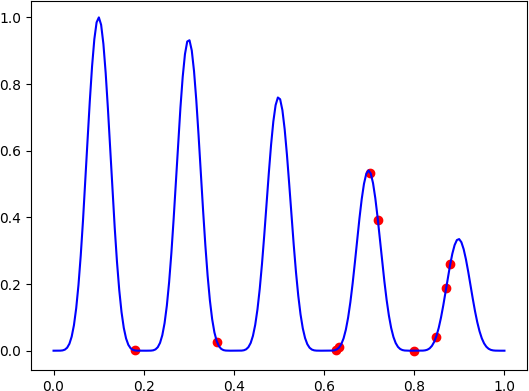
\includegraphics[width=0.65\textwidth]{images/p1_initial_hc}
\caption{Initial point distribution}
\label{fig:p1_initial}
\end{figure}

\newpage
\begin{figure}[H]
\centering
\noindent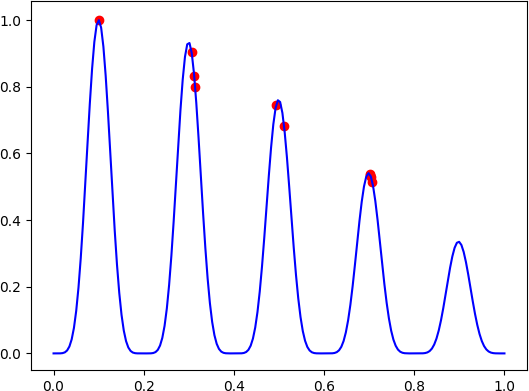
\includegraphics[width=0.65\textwidth]{images/p1_final_hc}
\caption{Points after Hill Climb algorithm}
\label{fig:p1_final}
\end{figure}

\newpage
\begin{figure}[H]
\centering
\noindent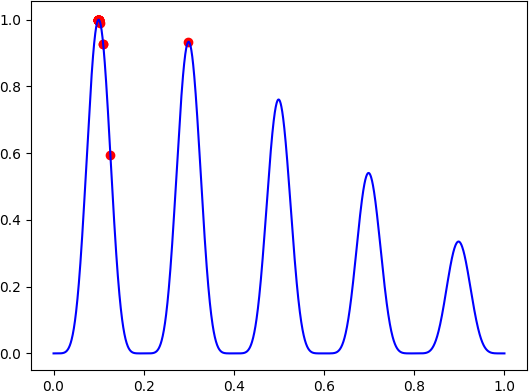
\includegraphics[width=0.65\textwidth]{images/p1_hc_hop}
\caption{Max points during Hill Climb algorithm}
\label{fig:p1_hop}
\end{figure}

\newpage
\begin{figure}[H]
\centering
\begin{minipage}{.45\textwidth}
  \centering
  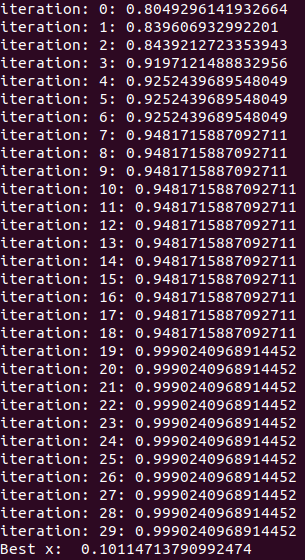
\includegraphics[width=.95\linewidth]{images/p1_iterations_hc}
  \caption{Maximum values at each iteration/generation}
  \label{fig:p1_iter}
\end{minipage}\hfill
\begin{minipage}{.45\textwidth}
  \centering
  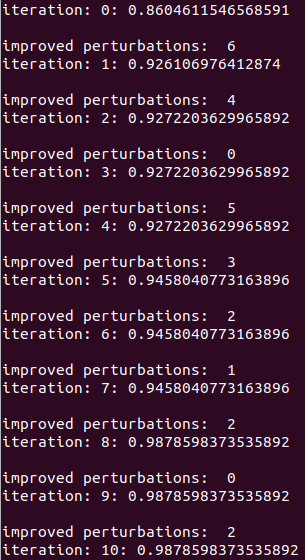
\includegraphics[width=.95\linewidth]{images/p1_perturbations_hc}
  \caption{Perturbations better than their original values. Float value represents fitness.}
  \label{fig:p1_pert}
\end{minipage}
\end{figure}

\newpage
\begin{figure}[H]
\centering
\begin{minipage}{.45\textwidth}
  \centering
  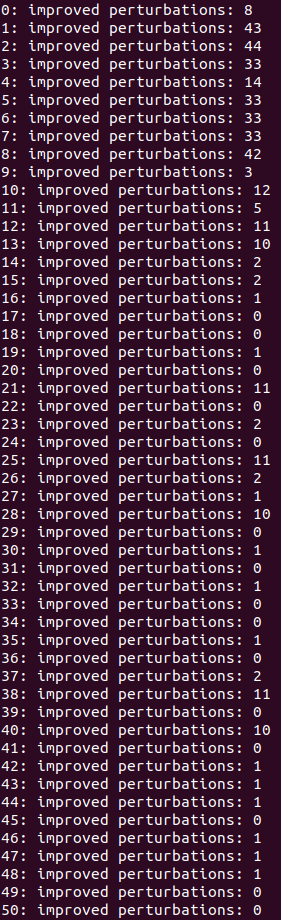
\includegraphics[width=.75\linewidth]{images/p1_sa2}
  \caption{T updated with T = T * 0.9}
  \label{fig:p1_sa2}
\end{minipage}\hfill
\begin{minipage}{.45\textwidth}
  \centering
  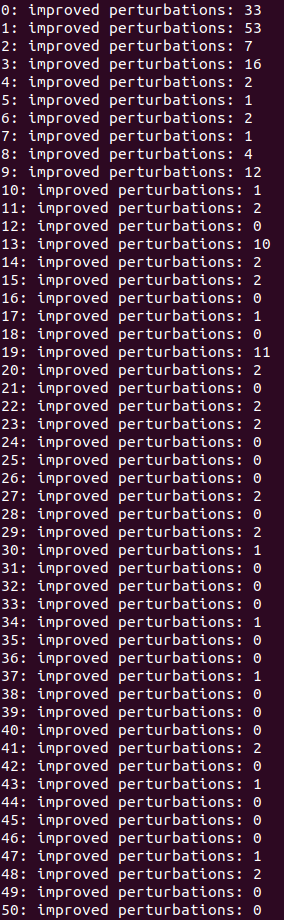
\includegraphics[width=.75\linewidth]{images/p1_sa3}
  \caption{T updated with T = T * 0.8}
  \label{fig:p1_sa3}
\end{minipage}
\end{figure}

\newpage
\begin{figure}[H]
\centering
\noindent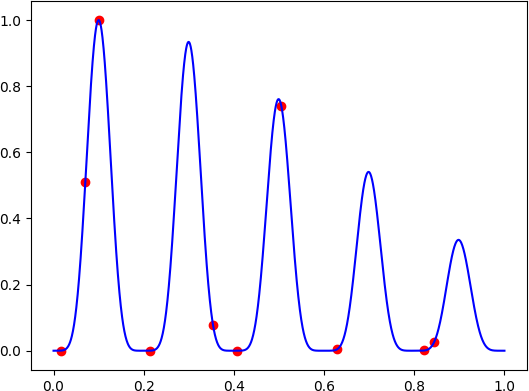
\includegraphics[width=0.65\textwidth]{images/p1_initial_sa}
\caption{Initial point distribution}
\label{fig:p1_initial_sa}
\end{figure}

\newpage
\begin{figure}[H]
\centering
\noindent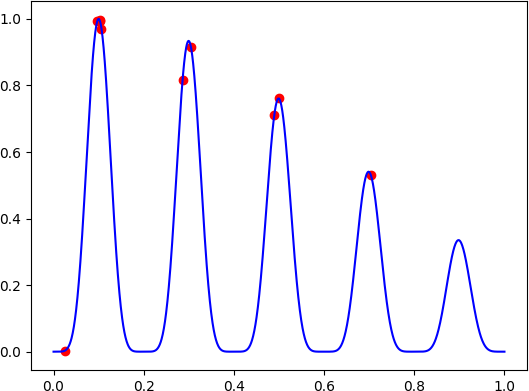
\includegraphics[width=0.65\textwidth]{images/p1_final_sa}
\caption{Points after Simulated Annealing algorithm}
\label{fig:p1_final_sa}
\end{figure}

\newpage
\begin{figure}[H]
\centering
\noindent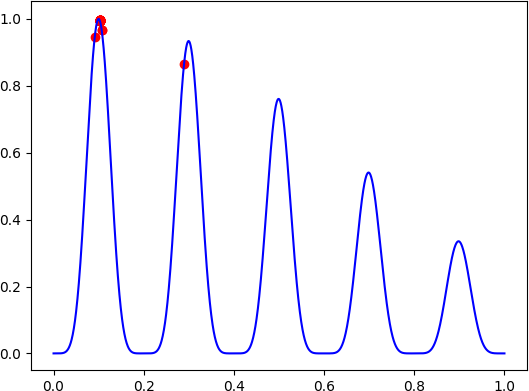
\includegraphics[width=0.65\textwidth]{images/p1_hop_sa}
\caption{Max points during Simulated Annealing algorithm}
\label{fig:p1_hop_sa}
\end{figure}


\newpage
\subsection{Code}
\subsubsection{Hill Climb}
\begin{lstlisting}
import numpy as np
import matplotlib.pyplot as plt


class GA():
    def __init__(self, pool=10, generations=10, debug=False):
        self.pool = pool
        self.generations = generations
        self.debug = debug
        self.t = 0
        self.max_iter = 30
        self.InitializeX()

    def reset(self):
        self.x = np.copy(self.og)
        self.t = 0

    def InitializeX(self):
        self.og = np.random.uniform(0, 1, size=(1, self.pool))
        self.x = np.copy(self.og)
        self.function = np.linspace(0, 1, 2000)
        self.function = self.EvalX(self.function)
        self.max = np.zeros(self.max_iter)
        self.max_fitness = np.zeros(self.max_iter)

    def Eval(self):
        self.fitness = np.power(2, -2 * ((self.x - 0.1) / 0.9)**2) * 
                       (np.sin(5 * np.pi * self.x)**6)
        # Make self.X a 2D array [x, fitness]
        self.X = np.concatenate((self.x, self.fitness), axis=0)
        # Sort and flip so the fitness is in order
        self.X = np.flip(np.argsort(self.X, axis=1))
        if self.debug:
            print('iteration: {}: {}\n'.
                format(self.t, self.fitness[0][self.X[0][0]]))
        # Note:
        # self.X is now in [fitness, x] order

    def EvalX(self, x):
        return np.power(2, -2 * ((x - 0.1) / 0.9)**2) *
               (np.sin(5 * np.pi * x)**6)

    def Draw(self):        
        plt.scatter(self.x, self.fitness, color='r', marker='o')
        plt.plot(np.linspace(0, 1, 2000), self.function, color='b')
        plt.show()

    def DrawMax(self):
        plt.scatter(self.max, self.max_fitness, color='r', marker='o')
        plt.plot(np.linspace(0, 1, 2000), self.function, color='b')
        plt.show()

    def SetMax(self):
        self.max[self.t] = self.x[0][self.X[0][0]]
        self.max_fitness[self.t] = self.fitness[0][self.X[0][0]]

    def MainLoopHC(self):
        self.Eval()
        self.SetMax()
        self.Draw()
        self.t = 1
        while (self.t < self.max_iter):
            self.PerturbX()
            self.Eval()
            self.SetMax()
            self.t += 1
        self.X = np.flip(self.X)
        self.Draw()
        self.DrawMax()
        print('Best x: ', self.x[0][self.X[0][0]])

    def PerturbX(self, sa=False):
        count = 0
        for i in range(self.pool):
            modifier = np.abs(np.random.normal(0, 0.25, 1) * 
                              self.x[0][i] + self.x[0][i])
            # If the fitness of the modified value > x, x = modified
            if self.fitness[0][i] < self.EvalX(modifier):
                self.x[0][i] = modifier
                count += 1
        if self.debug:
            print('improved perturbations: ', count)

    def Run(self):
        self.MainLoopHC()
        self.reset()

if __name__ == '__main__':
    ga = GA()
    ga.Run()
\end{lstlisting}

\newpage
\subsubsection{Simulated Annealing}
\begin{lstlisting}
import numpy as np
import matplotlib.pyplot as plt


class GA():
    def __init__(self, pool=10, generations=10, debug=False):
        self.pool = pool
        self.generations = generations
        self.debug = debug
        self.state = 'hc'
        self.max_iter = 30
        self.InitializeX()

    def reset(self):
        self.x = np.copy(self.og)
        self.InitializeT()

    def InitializeX(self):
        self.og = np.random.uniform(0, 1, size=(1, self.pool))
        self.reset()
        self.function = np.linspace(0, 1, 2000)
        self.function = self.EvalX(self.function)
        self.max = np.zeros(self.max_iter)
        self.max_fitness = np.zeros(self.max_iter)

    def InitializeT(self):
        if self.state == 'hc':
            self.t = 0
        else:
            self.t = 0.25

    def UpdateT(self):
        if self.state == 'hc':
            self.t += 1
        else:
            self.t *= 0.8

    def Eval(self):
        self.fitness = np.power(2, -2 * ((self.x - 0.1) / 0.9)**2) * 
                                (np.sin(5 * np.pi * self.x)**6)
        # Make self.X a 2D array [x, fitness]
        self.X = np.concatenate((self.x, self.fitness), axis=0)
        # Sort and flip so the fitness is in order
        self.X = np.flip(np.argsort(self.X, axis=1))
        if self.debug:
            print('iteration: {}: {}\n'.
                format(self.t, self.fitness[0][self.X[0][0]]))
        # Note:
        # self.X is now in [fitness, x] order

    def EvalX(self, x):
        return np.power(2, -2 * ((x - 0.1) / 0.9)**2) * 
               (np.sin(5 * np.pi * x)**6)

    def EvalXSA(self, x):
        ret_val = np.power(2, -2 * ((x - 0.1) / 0.9)**2) *
                  (np.sin(5 * np.pi * x)**6)
        if ret_val > 1 or ret_val < 0:
            return -1000
        else:
            return ret_val

    def EvalSA(self):
        self.fitness = np.power(2, -2 * ((self.x - 0.1) / 0.9)**2) *
                       (np.sin(5 * np.pi * self.x)**6)
        self.max_index = np.argsort(-self.fitness)[0][0]

    def Draw(self):        
        plt.scatter(self.x, self.fitness, color='r', marker='o')
        plt.plot(np.linspace(0, 1, 2000), self.function, color='b')
        plt.show()

    def DrawMax(self):
        plt.scatter(self.max, self.max_fitness, color='r', marker='o')
        plt.plot(np.linspace(0, 1, 2000), self.function, color='b')
        plt.show()

    def SetMaxSA(self):
        self.max[self.iteration] = self.x[0][self.max_index]
        self.max_fitness[self.iteration] = self.fitness[0][self.max_index]
        
    def MainLoopSA(self):
        self.state = 'sa'
        self.reset()
        self.iteration = 0
        self.EvalSA()
        self.SetMaxSA()
        self.Draw()
        while (self.iteration < self.max_iter):
            self.PerturbX()
            self.EvalSA()
            self.SetMaxSA()
            self.UpdateT()
            self.iteration += 1
        print('Best x: ', self.x[0][self.max_index])
        self.Draw()
        self.DrawMax()

    def PerturbX(self):
        count = 0
        for i in range(self.pool):
            modifier = np.abs(np.random.normal(0, 0.25, 1) * 
                              self.x[0][i] + self.x[0][i])
            fitness = self.EvalXSA(modifier)
            # If the fitness of the modified value > x, x = modified
            if self.fitness[0][i] < fitness:
                self.x[0][i] = modifier
                count += 1
            elif self.state == 'sa' and 
                               (np.random.random_sample() < 
                               np.exp(-np.abs(
                               self.fitness[0][i] - fitness) / self.t)):
                self.x[0][i] = modifier
                # 10 to differentiate
                count += 10
        if self.debug:
            print('{}: improved perturbations: {}'.format(self.iteration,
                                                          count))

    def Run(self):
        self.MainLoopSA()


if __name__ == '__main__':
    ga = GA()
    ga.Run()
\end{lstlisting}

\newpage
\section{}
\subsection{Statement}
In lecture we addressed the Traveling Salesman Problem using Simulated 
Annealing. To speed up convergence and increase the odds of finding the global 
extremal, it makes sense to try an evolutionary algorithm. The mutation operator 
can be adapted from the SA algorithm. Skip recombination in this problem. Write 
an evolutionary algorithm to solve the TSP as generated in the sample program. 
Compare deterministic and stochastic selection operators. 

\subsection{Experiments}
A deterministic approach will use strictly rank to determine the next 
generation, whereas a stochastic approach will use some form of randomness. I 
assume the best approach is going to be stochastic where rank determines 
probability of being accepted.

$$$$


Deterministic TSP:
\begin{algorithmic}
\STATE $gen = 0$
\STATE $epoch = 0$
\STATE Initialize($temperature$)
\STATE Initialize($tour$)
\STATE Eval($tour$)
\STATE Rank($tour$)
\WHILE   {$temperature > 0.001$}
\STATE   $cities' = $ SwapCity($(gen * 2) \%\ rollover$, $(gen * 2 + 1 + epoch)\%\ rollover$)
\STATE   Eval($tour$)
\STATE   Rank($tour$)
\IF      {Accept($tour$)}
\STATE     $cities = cities'$
\ENDIF
\STATE   $gen++$
\IF      {$gen \%\ rollover - 2 = 0 $}
\STATE     $epoch++$
\ENDIF
\STATE   UpdateTemp($temperature$)
\ENDWHILE
\end{algorithmic}

$$$$

I would have preferred to take a much different approach:
Set 50 tours as the pool. The top 5 cities will be kept through 
Elitism. The bottom 5 cities will be kept through ``Derpism''. The middle 40 
will go through 25 generations of city swaps. So cities 1, 2 swap on all 40 
cities and are then evaluated and ranked. Top/Bottom 5 are kept and the next 
generation swaps cities 3, 4. This happens until 25 generations have been 
completed. I decided ``Derpism'' is something might be good because it is possible 
that as those cities get pushed out of the bottom tier they may generate better 
solutions. \textit{I thought of it as a way to inject ``random'' into a 
deterministic approach.}

$$$$

That approach would have taken a lot more time than I had so I am keeping it in 
my back pocket for later. To address the problem statement I utilized the 
existing code for TSP\_SA and made the swap function either deterministic or 
stochastic. For the deterministic solution I settled on:

$$cities' = SwapCity((gen * 2) \%\ rollover, (gen * 2 + 1 + epoch)\%\ rollover)$$

$$$$

The stochastic solution simply performed a random swap on cities. 

\subsection{Results}

\newpage
\begin{figure}[H]
\centering
\begin{minipage}{.45\textwidth}
  \centering
  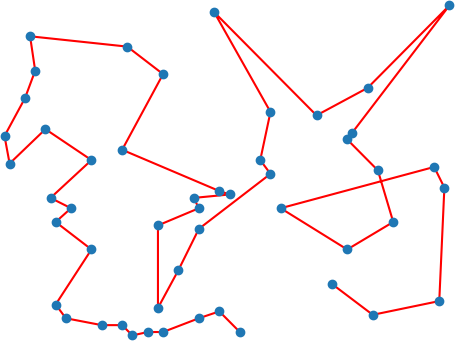
\includegraphics[width=.75\linewidth]{images/p2_det_1}
  \caption{Deterministic tour}
  \label{fig:p2_det_1}
\end{minipage}\hfill
\begin{minipage}{.45\textwidth}
  \centering
  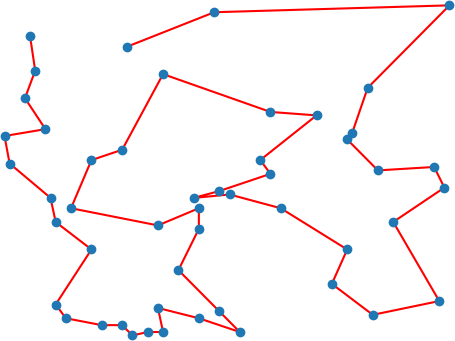
\includegraphics[width=.75\linewidth]{images/p2_stoch_1}
  \caption{Stochastic tour}
  \label{fig:p2_stoch_1}
\end{minipage}
\end{figure}


\begin{figure}[H]
\centering
\begin{minipage}{.45\textwidth}
  \centering
  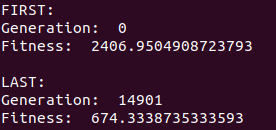
\includegraphics[width=.75\linewidth]{images/p2_det_2}
  \caption{Deterministic tour distance}
  \label{fig:p2_det_2}
\end{minipage}\hfill
\begin{minipage}{.45\textwidth}
  \centering
  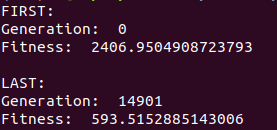
\includegraphics[width=.75\linewidth]{images/p2_stoch_2}
  \caption{Stochastic tour distance}
  \label{fig:p2_stoch_2}
\end{minipage}
\end{figure}

$$$$

As can be seen in Figure \ref{fig:p2_stoch_2}, a stochastic algorithm 
outperformed deterministic (as shown in Figure \ref{fig:p2_det_2}). Figure 
\ref{fig:p2_det_1} and Figure \ref{fig:p2_stoch_1} show the final tours of the 
algorithms. I locked the random and numpy random seeds to set values and then 
tested both a dozen times with a different seed for each test. Stochastic 
outperformed deterministic almost every time, which was expected. There are 
deterministic solutions that will be better than random depending on the layout 
of cities and the deterministic solution. In something like TSP some measure of 
a stochastic approach seems to fare better. Playing around with the order of 
swaps didn't seem to yield any one ``better'' solution. I would have needed to 
test a statistically significant amount of runs to determine if one ordering was 
better than another on this given city size. Would have been a good graduate 
bonus I guess. 

``Does an array invert before or after the swap make for a better TSP solution?''


\newpage
\subsection{Code}
\begin{lstlisting}
def swap_rand(x):
    i = random.randint(0, len(x) - 2)
    j = random.randint(i, len(x) - 1)

    y = np.copy(x)
    y[i: j] = y[i: j][::-1]

    return y

def swap(x, gen, epoch):
    i = (gen * 2) % 50
    j = (gen * 2 + 1 + epoch) % 50
    y = np.copy(x)
    y[i: j] = y[i: j][::-1]
    temp = np.copy(y[i])
    y[i] = np.copy(y[j])
    y[j] = np.copy(temp)
    return y

def run(cities, cities_number, temperature = 800, cooling_factor = .001):
    current = evaluate(cities)
    i = 0
    gen = 0
    epoch = 0
    while temperature > 0.001:
        if gen == 0:
            print('FIRST:')
            print('Generation: ', gen)
            print('Fitness: ', current)
            print()
        new_solution = swap(cities, gen, epoch)
        # new_solution = swap_rand(cities)
        energy = evaluate(new_solution)
        if accept_solution(current, energy, temperature):
            cities = new_solution
            current = energy

        

        if (i%50==0):
            plot(cities,path = 1, wait = 0)
        if gen == 14901:
            print('LAST:')
            print('Generation: ', gen)
            print('Fitness: ', current)
            print()

        temperature *= 1 - cooling_factor
        i = i+1
        gen += 1
        if gen % 50 - 2 == 0:
            epoch += 1
    return cities
\end{lstlisting}

\newpage
\section{} %%  This will generate a numbered problem header.

\subsection{Statement}
In problem 2, we implemented EA code to solve the Traveling Salesman Problem. 
In this problem, implement recombination (crossover) in your EA. For this 
problem you will need to use an encoding that prevents crossover that creates 
an invalid candidate. As before, compare deterministic and stochastic selection 
operators.

\subsection{Method}
I would like to try something I am calling the Starfish Approach. This is a 
two-part approach that involves recombination and mutation. I'll attempt both 
deterministic and stochastic approaches. 

$$$$

Chop off a starfish's leg and a new starfish will grow from it if part of the 
central disk is attached to that leg. The removed leg will regrow as well. 
In this case I intend reproduction through chopping up the best solution into 
ten parts. One ``leg'' (10 cities) will be removed from each copy of the best 
solution. Each amputated leg will be regrown with a mutation. Each body will be 
regrown with a mutation. All ten of the new starfish will be evaluated and the 
best will be kept for the next generation. So there are five bodies and five 
legs that will undergo mutation for a pool of 10 starfish to evaluate.

$$$$

A ``standard'' crossover could be obtained by simply swapping the arms that 
were cut off but that is boring. I used an asexual reproduction approach. 
Also, I like the idea of the arm growing back with a mutation. When DNA is 
replicated there is opportunity for mutation. 


\subsection{Results}

\begin{figure}[H]
\centering
\begin{minipage}{.45\textwidth}
  \centering
  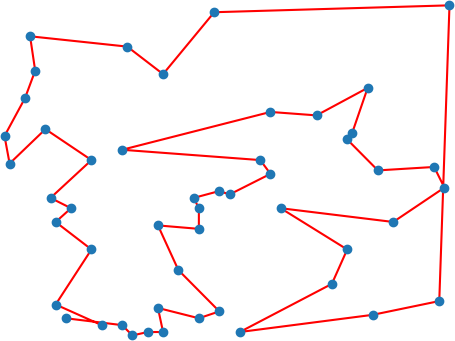
\includegraphics[width=.75\linewidth]{images/p2_star_det_1}
  \caption{Deterministic Starfish tour distance}
  \label{fig:p2_star_det_1}
\end{minipage}\hfill
\begin{minipage}{.45\textwidth}
  \centering
  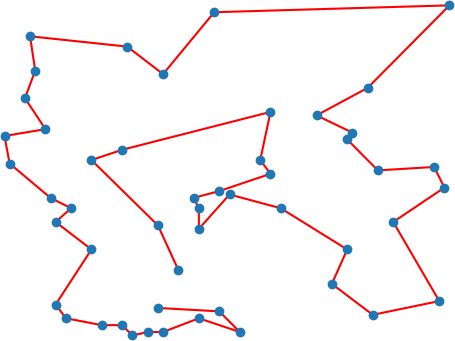
\includegraphics[width=.75\linewidth]{images/p2_star_stoch_1}
  \caption{Stochastic Starfish tour distance}
  \label{fig:p2_star_stoch_1}
\end{minipage}
\end{figure}

\begin{figure}[H]
\centering
\begin{minipage}{.45\textwidth}
  \centering
  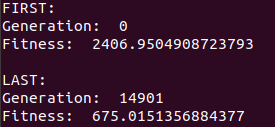
\includegraphics[width=.75\linewidth]{images/p2_star_det_2}
  \caption{Deterministic Starfish path}
  \label{fig:p2_star_det_2}
\end{minipage}\hfill
\begin{minipage}{.45\textwidth}
  \centering
  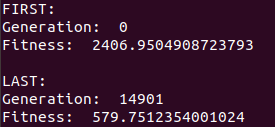
\includegraphics[width=.75\linewidth]{images/p2_star_stoch_2}
  \caption{Stochastic Starfish path}
  \label{fig:p2_star_stoch_2}
\end{minipage}
\end{figure}

This method behaved about as expected and was incredibly slow. The slowness was 
to be expected because of all the array splicing and creation. The results of 
seeds 10-40 can be seen in the PDF in Section \ref{fig:starfish_results}. 17 
out of 40 times Starfish surpassed no recombination, 23 times out of 40 it 
failed. Perhaps more interesting would be that Starfish averaged a fitness of 
629 and no recombination averaged 611. 

$$$$

Watching the plot update I found Starfish was \textbf{much} quicker to start 
picking out a coherent path compared to previous methods. I believe this method 
has a lot of potential and that it would outperform all other methods by a good 
margin if more time were put into tweaking it. For one, the splicing always 
happening at regular points is a huge area for improvement. It would benefit 
from a pool of random splice points and sizes. Figure \ref{fig:p2_star_det_1} 
and Figure \ref{fig:p2_star_stoch_1} show the comparison between deterministic 
and stochastic selection of mutations. 

$$$$

\begin{center}
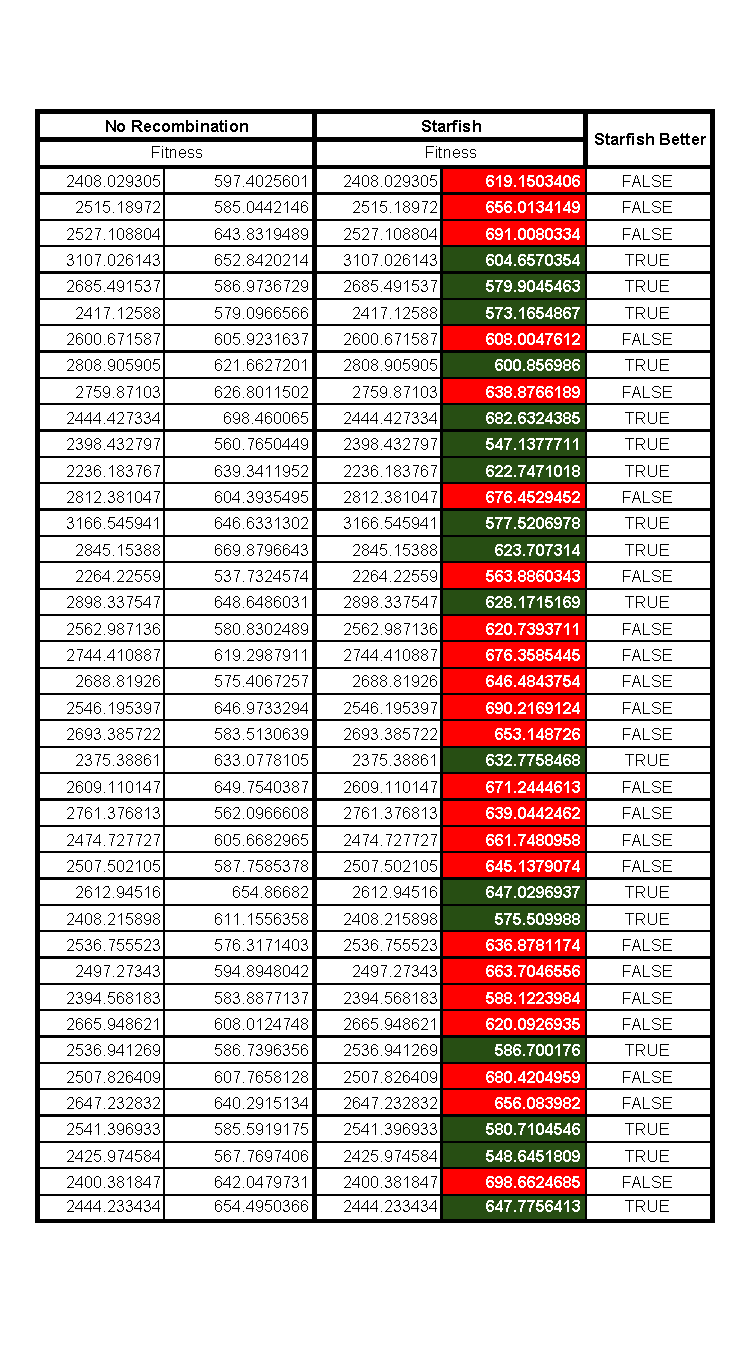
\includepdf[pages=-]{images/StarfishAnalysis.pdf}
\label{fig:starfish_results}
\end{center}

\newpage
\subsection{Code}
\begin{lstlisting}
import numpy as np
import matplotlib.pyplot as plt
import random
import math

#  Computer the tour length
def evaluate(cities):
    distance = 0
    for index in range(len(cities)):
        a = cities[index]
        if index == len(cities) - 1:
            b = cities[0]
        else:
            b = cities[index + 1]

        distance += np.linalg.norm(a - b)
        index += 1

    return distance

# A perturbation is a city swap
def swap_rand(x):
    i = random.randint(0, x.size - 2)
    j = random.randint(i, x.size - 1)

    y = np.copy(x)
    # swap cities and invert sublist
    y[i: j] = y[i: j][::-1]

    return y

def swap(x, gen, epoch):
    i = (gen * 2) % (x.size // 2)
    j = (gen * 2 + 1 + epoch) % (x.size // 2)
    y = np.copy(x)

    temp = np.copy(y[i])
    y[i] = np.copy(y[j])
    y[j] = np.copy(temp)
    y[i: j] = y[i: j][::-1]
    return y


def accept_solution(energy1, energy2, temperature):
    if energy1 > energy2:
        return True
    else:
        a = math.exp((energy1 - energy2) / temperature)
        b = random.random()
        if a > b:
            return True
        else:
            return False

def Reproduce(cities, det, gen, epoch):
    childbody = np.zeros((5, 40, 2), dtype=int)
    childleg = np.zeros((5, 10, 2), dtype=int)

    for i in range(5):
        bod_min = i * 10
        bod_max = bod_min + 10
        childbody[i] = np.concatenate([np.copy(cities[:bod_min, :]),
                                      np.copy(cities[bod_max:, :])], axis=0)
        # Take only the leg
        childleg[i] = np.copy(cities[bod_min:bod_max])

    cb, cl = Mutate(childbody, childleg, det, gen, epoch)
    y = Regrow(cb, cl, cities)
    return y

def Mutate(cb, cl, det, gen, epoch):
    if det:
        for i in range(5):
            cb[i] = swap(cb[i], gen, epoch)
            cl[i] = swap(cl[i], gen, epoch)
    else:
        for i in range(5):
            cb[i] = swap_rand(cb[i])
            cl[i] = swap_rand(cl[i])

    return cb, cl

def Regrow(cb, cl, x):
    y = np.zeros((10, 50, 2), dtype=np.int)
    for i in range(5):
        bod_min = i * 10
        bod_max = bod_min + 10
        y[i * 2] = np.copy(x)
        y[i * 2+ 1] = np.copy(x)
        # Body
        y[i, :bod_min, :] = cb[i, :bod_min, :]
        y[i, bod_max:, :] = cb[i, bod_min:, :]
        # Leg
        y[i + 1, bod_min:bod_max, :] = cl[i]

    return y


def run(cities, cities_number, temperature = 800, cooling_factor = .001):
    det = False
    current = evaluate(cities)
    i = 0
    gen = 0
    epoch = 0
    while temperature > 0.001:
        y = Reproduce(cities, det, gen, epoch)
        max_energy = current
        min_index = -1
        for j in range(10):
            energy = evaluate(y[j])
            if accept_solution(current, energy, temperature):
                cities = np.copy(y[j])
                current = energy
                if max_energy > current:
                    max_energy = current
                    min_index = j

        # Overcomes energy mixups
        if min_index != -1:
            cities = np.copy(y[min_index])
            current = max_energy

        if (i%50==0):
            plot(cities,path = 1, wait = 0)

        temperature *= 1 - cooling_factor
        i = i+1
        gen += 1
        if gen % 50 - 2 == 0:
            epoch += 1
    return cities


def plot(cities, path, wait):
    plt.clf()
    if (path == 1):
        plt.plot(cities[:, 0], cities[:, 1], color='red', zorder=0)
    plt.scatter(cities[:, 0], cities[:, 1], marker='o')
    plt.axis('off')
    if (wait == 0):  plt.ion()
    plt.show()
    plt.pause(.001)

print()
cities_number = 50
for i in range(10):
    seed = i
    random.seed(seed)
    np.random.seed(seed)
    cities = (np.random.rand(cities_number, 2) * 100).astype(int)
    plot(cities,path = 0, wait = 1)
    cities = run(cities, cities_number, temperature = 3000)
    plt.ioff()
    plot(cities,path = 1, wait = 1)

print()
\end{lstlisting}

 \end{document}
